\documentclass[12pt,fleqn]{article}\usepackage{../../common}
\begin{document}
Frekanslar, Uygulamalar

Ad�m �l�mek, Pedometre

\begin{minted}[fontsize=\footnotesize]{python}
import pandas as pd
dfacc = pd.read_csv('acc.txt',header=None,sep='\s+')
print dfacc.head()
\end{minted}

\begin{verbatim}
               0         1         2         3
0  1493818386218 -0.147100  6.972528  6.707748
1  1493818386422 -0.215746  7.001948  6.854848
2  1493818386610 -0.304006  7.041174  6.697942
3  1493818386812 -0.304006  7.050981  6.884268
4  1493818387008 -0.225553  7.011754  6.943108
\end{verbatim}

\begin{minted}[fontsize=\footnotesize]{python}
steps1 = np.sqrt(np.sum(dfacc[[1,2,3]]**2, axis=1))
steps2 = steps1 - 10.0
steps2[:200].plot()
plt.savefig('compscieng_app60wave_01.png')
\end{minted}

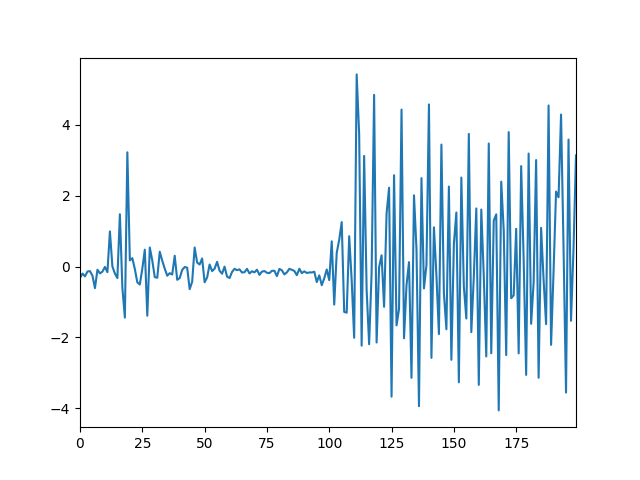
\includegraphics[height=6cm]{compscieng_app60wave_01.png}

\begin{minted}[fontsize=\footnotesize]{python}
fs = 6
fou = np.fft.fft(steps1, fs)
hmag=np.real(fou); ah=hmag/len(steps1);
f=plt.figure()
plt.stem(ah)
plt.savefig('compscieng_app60wave_02.png')

f=plt.figure()
fou = np.fft.fft(steps2, fs)
hmag=np.real(fou); ah=hmag/len(steps2);
f=plt.figure()
plt.stem(ah)
plt.savefig('compscieng_app60wave_06.png')
\end{minted}

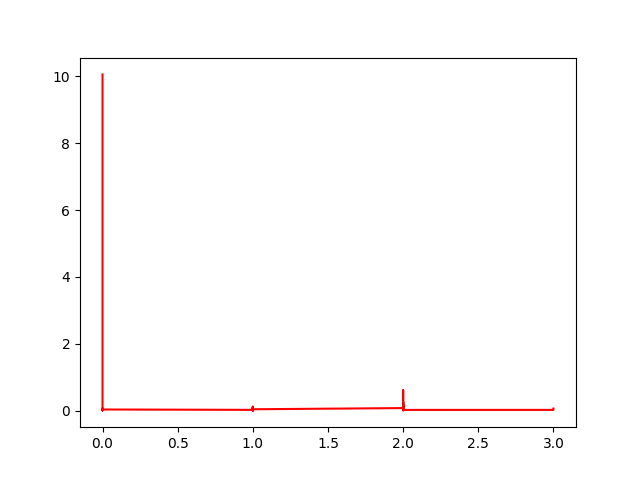
\includegraphics[height=6cm]{compscieng_app60wave_02.png}
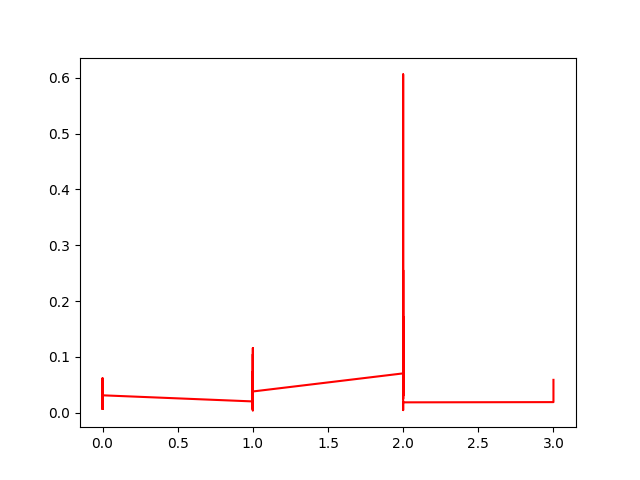
\includegraphics[height=6cm]{compscieng_app60wave_06.png}

\begin{minted}[fontsize=\footnotesize]{python}
import sys; sys.path.append('../tser_freq1')
import filt, peakutils
bp = filt.sinc_filter_band(32, 1.0, 4.0, fs);
bpSteps = np.convolve(bp, steps2)
f=plt.figure()
plt.plot(bpSteps[200:300])
plt.savefig('compscieng_app60wave_04.png')
f=plt.figure()
plt.plot(steps2[200:300])
plt.savefig('compscieng_app60wave_05.png')
\end{minted}

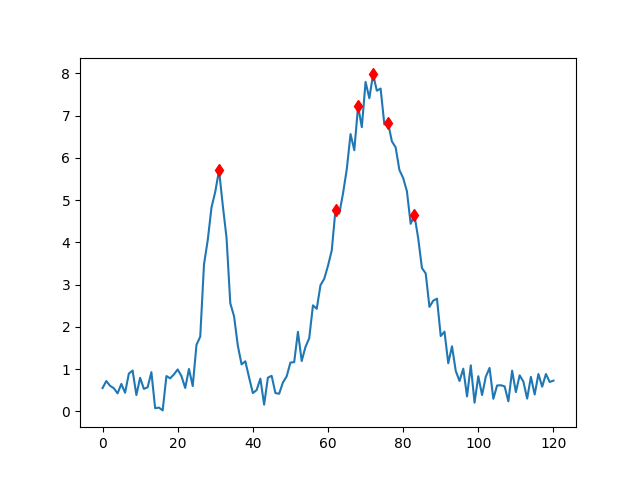
\includegraphics[height=6cm]{compscieng_app60wave_05.png}
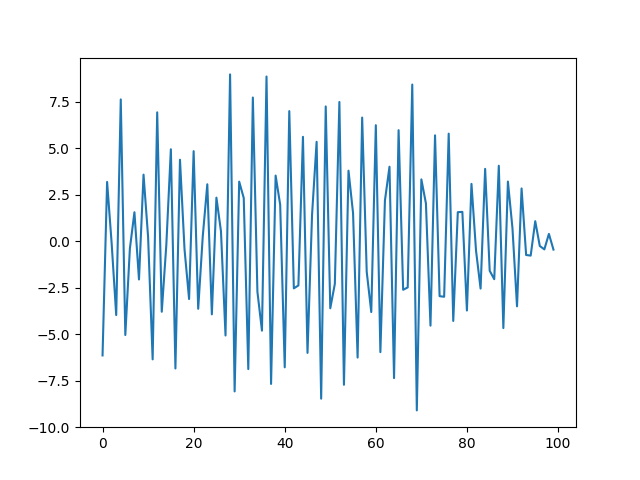
\includegraphics[height=6cm]{compscieng_app60wave_04.png}

\begin{minted}[fontsize=\footnotesize]{python}
idx = peakutils.indexes(bpSteps, thres=0.1, min_dist=3)
print len(idx)
plt.plot(bpSteps)
plt.plot(idx,bpSteps[idx],'rd')
plt.savefig('compscieng_app60wave_03.png')
\end{minted}

\begin{verbatim}
89
\end{verbatim}

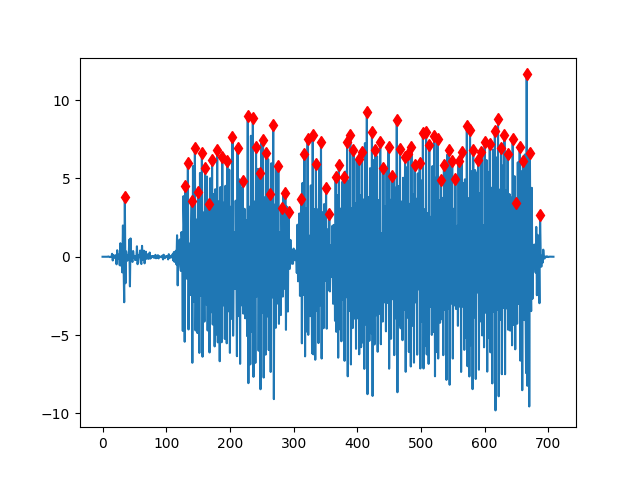
\includegraphics[height=6cm]{compscieng_app60wave_03.png}

\begin{minted}[fontsize=\footnotesize]{python}
idx2 = peakutils.indexes(steps2, thres=0.1, min_dist=3)
print len(idx2)
\end{minted}

\begin{verbatim}
89
\end{verbatim}

85*2 = 160 adim olmali

Radyo Dalgalari

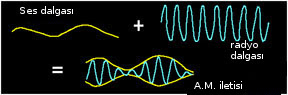
\includegraphics[width=20em]{AM_waves.jpg}

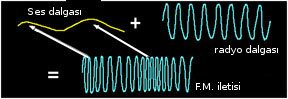
\includegraphics[width=20em]{FM_waves.jpg}

\begin{minted}[fontsize=\footnotesize]{python}
import numpy as np
import matplotlib.pyplot as plt
import scipy.signal as signal
dir = "/home/burak/Documents/Dropbox/Public/data"
extract_data = np.fromfile(dir + "/fm1.dat",dtype="uint8")
interleavedData = extract_data[0::2] + 1j*extract_data[1::2]
\end{minted}

\begin{minted}[fontsize=\footnotesize]{python}
plt.title("SpectoGram of 'signal' loaded from file")
plt.xlabel("Time")
plt.ylabel("Frequency")
plt.specgram(interleavedData, NFFT =1024, Fs=1140000)
plt.savefig('compscieng_app60wave_07.png')
\end{minted}

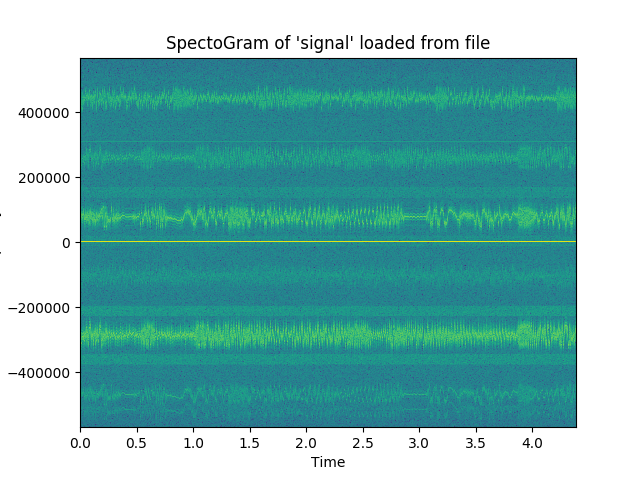
\includegraphics[width=20em]{compscieng_app60wave_07.png}

\begin{minted}[fontsize=\footnotesize]{python}
plt.title("PSD of interleaved Data")
plt.psd(interleavedData, NFFT=1024, Fs=1140000)
plt.savefig('compscieng_app60wave_08.png')
\end{minted}

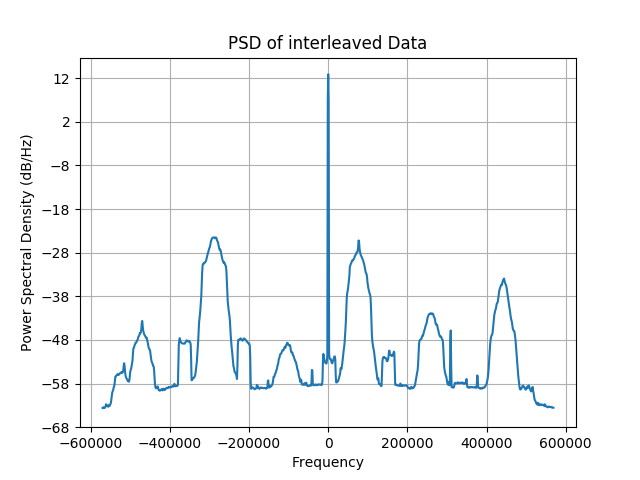
\includegraphics[width=20em]{compscieng_app60wave_08.png}

\begin{minted}[fontsize=\footnotesize]{python}
calculate_range = max(interleavedData) - min(interleavedData);
data = (interleavedData - min(interleavedData))/ calculate_range
x1 = (data*2) - 1
plt.title("SpectoGram of signal post normalization")
plt.xlabel("Time")
plt.ylabel("Frequency")
plt.specgram(x1, NFFT =1024, Fs=1140000)
plt.savefig('compscieng_app60wave_09.png')
\end{minted}

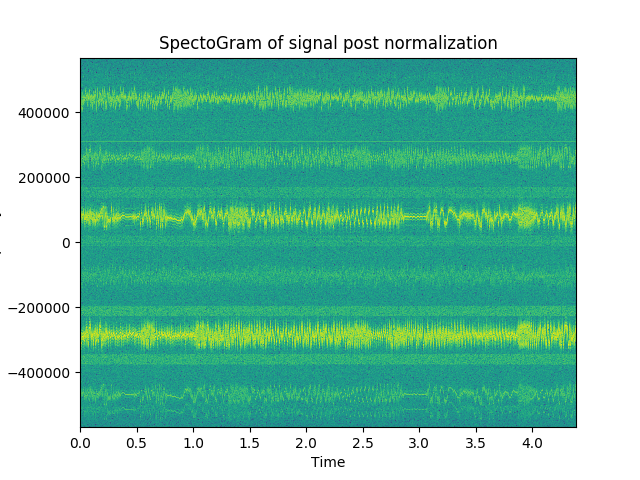
\includegraphics[width=20em]{compscieng_app60wave_09.png}

\begin{minted}[fontsize=\footnotesize]{python}
plt.title("PSD of normalized signal")
plt.psd(x1, NFFT=1024, Fs=1140000)
plt.savefig('compscieng_app60wave_10.png')
\end{minted}

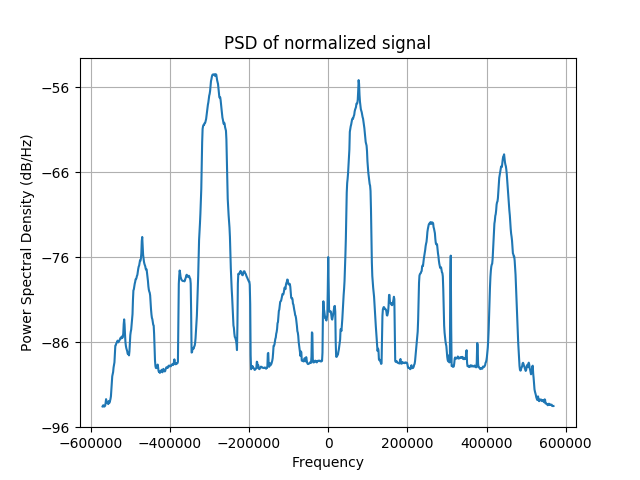
\includegraphics[width=20em]{compscieng_app60wave_10.png}

\begin{minted}[fontsize=\footnotesize]{python}
Fs = 1140000
fc = np.exp(-1.0j*2.0*np.pi* 250000/Fs*np.arange(len(x1)))
x2 = x1*fc
f_bw=200000
Fs=1140000
n_taps=64
lpf= signal.remez(n_taps, [0, f_bw, f_bw +(Fs/2-f_bw)/4,Fs/2], [1,0], Hz=Fs)
w,h = signal.freqz(lpf)
x3 = signal.lfilter(lpf, 1.0, x2)
dec_rate = int(Fs/f_bw)
x4 = signal.decimate(x3, dec_rate)
Fs_x4 = Fs/dec_rate
y = x4[1:] * np.conj(x4[:-1])

x5 = np.angle(y)
d = Fs_x4 * 75e-6   # Calculate the # of samples to hit the -3dB point
r = np.exp(-1/d)   # Calculate the decay between each sample
b = [1-r]          # Create the filter coefficients
a = [1,-r]
x6 = signal.lfilter(b,a,x5)

d = Fs_x4 * 75e-6   # Calculate the # of samples to hit the -3dB point
r = np.exp(-1/d)   # Calculate the decay between each sample
b = [1-r]          # Create the filter coefficients
a = [1,-r]
dec_rate = int(Fs/f_bw)
x7=signal.decimate(x6,dec_rate)
x7*= 10000 / np.max(np.abs(x7))               # scale so it's audible
x7.astype("int16").tofile("radio.raw")
\end{minted}


\begin{verbatim}
aplay radio.raw -r 100000.0 -f S16_LE -t raw -c 1
\end{verbatim}

\begin{verbatim}
aplay radio.raw -r 45600 -f S16_LE -t raw -c 1
\end{verbatim}

[devam edecek]

Kaynaklar

[1] {\em The Basic Facts About Radio Signals}, \url{https://www.windows2universe.org/spaceweather/wave_modulation.html}

[2] \url{https://www.dropbox.com/s/lpwz2iby0nhh8p7/fm1.dat?dl=1}

[3] \url{https://www.dropbox.com/s/70adji6wyst0qbi/fm2.dat?dl=1}

[4] Scher, {\em How to capture raw IQ data from a RTL-SDR dongle and FM demodulate with MATLAB},\url{http://www.aaronscher.com/wireless_com_SDR/RTL_SDR_AM_spectrum_demod.html}

[5] {\em EE123: Digital Signal Processing}, \url{http://inst.eecs.berkeley.edu/~ee123/sp14/}

[6] Fund, {\em Capture and decode FM radio}, \url{https://witestlab.poly.edu/blog/capture-and-decode-fm-radio/}

[7] Fund, {\em Lab 1: Working with IQ data in Python}, \url{http://witestlab.poly.edu/~ffund/el9043/labs/lab1.html}

[8] Barton, {\em Nest Interview}, \url{https://github.com/sbarton272/Pedometer}

\end{document}


